\documentclass[a4paper, 12pt]{article} % тип документа

%%%Библиотеки
	%\usepackage[warn]{mathtext}	
	\usepackage[T2A]{fontenc}   %Кодировка
	\usepackage[utf8]{inputenc} %Кодировка исходного текста
	\usepackage[english, russian]{babel} %Локализация и переносы
	\usepackage{caption}
	\usepackage{listings}
	\usepackage{amsmath, amsfonts, amssymb, amsthm, mathtools}
	\usepackage[warn]{mathtext}
	\usepackage[mathscr]{eucal}
	\usepackage{wasysym}
	\usepackage{graphicx} %Вставка картинок правильная
	\DeclareGraphicsExtensions{.pdf,.png,.jpg}
	\graphicspath{ {images/} }
	
	\setlength{\parskip}{0.5cm}
	
	\usepackage{pgfplots}
	\usepackage{indentfirst}
	\usepackage{float}    %Плавающие картинки
	\usepackage{wrapfig}  %Обтекание фигур (таблиц, картинок и прочего)
	\usepackage{fancyhdr} %Загрузим пакет
	\usepackage{lscape}
	\usepackage{xcolor}
	\usepackage[normalem]{ulem}
	\usepackage{wasysym}
	
	\usepackage{titlesec}
	\titlelabel{\thetitle.\quad}

	\usepackage{hyperref}
	\newenvironment{comment}{}{}

%%%Конец библиотек

%%%Настройка ссылок
	\hypersetup
	{
		colorlinks = true,
		linkcolor  = blue,
		filecolor  = magenta,
		urlcolor   = blue
	}
%%%Конец настройки ссылок


%%%Настройка колонтитулы
	\pagestyle{fancy}
	\fancyhead{}
	\fancyhead[L]{2.4.1}
	\fancyhead[R]{Старченко Иван, группа Б01-005}
	\fancyfoot[C]{\thepage}
%%%конец настройки колонтитулы

\begin{document}
\setcounter{page}{1}

\begin{center}
  \LARGE{Лабораторная работа 3.4.5}\\[0.2cm]
  \LARGE{Петля гистерезиса(динамический метод).}\\[0.2cm]
  \large{16 октября 2021 г.}\\[0.2cm]
  \large{Старченко Иван Александрович}\\[0.2cm]
\end{center}

\textbf{Цель работы:} изучение петель гистерезиса различных ферромагнитных
материалов в переменных полях.
\\

\textbf{Оборудование:} автотрансформатор, понижающий трансформатор, интегрирующая цепочка, амперметр, вольтметр, электронный
осциллограф, делитель напряжения, тороидальные образцы с двумя обмотками.

\section{Теория}
Основные характеристики
ферромагнетиков — их коэрцитивное поле $H_c$, магнитная проницаемость
$\mu$, рассеиваемая в виде тепла при перемагничивании мощность — зависят
от частоты перемагничивающего поля. В данной работе кривые гистерезиса ферромагнитных материалов изучаются в поле частоты $\nu_0$ = 50 Гц
с помощью электронного осциллографа.
\begin{figure}[h!]
    \centering
    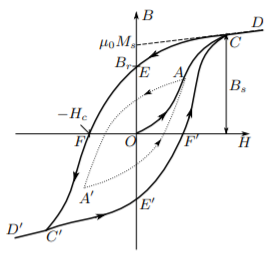
\includegraphics{petlya.png}
    \caption{Петля гистерезиса ферромагнетика}
    \label{fig:petlya}
\end{figure}

Магнитная индукция B и напряжённость поля H в ферромагнитном материале неоднозначно связаны между собой: индукция зависит
не только от напряжённости, но и от предыстории образца. Связь между B и H типичного ферромагнетика иллюстрирует Рис. $\ref{fig:petlya}$.

Если к ферромагнитному образцу прикладывать переменное внешнее
магнитное поле, то его состояние на плоскости B-H будет изменяться
по замкнутой кривой — петле гистерезиса. Размер петли определяется
максимальным значением напряжённости H в цикле (например, петля AA',
обозначенная пунктиром на Рис. $\ref{fig:petlya}$). Если амплитуда напряжённости достаточно велика, то образец будет периодически достигать насыщения,
что на рисунке соответствует кривой CEFC'E'F'C (предельная петля
гистерезиса). Пересечение предельной петли с вертикальной осью соответствует остаточной индукции $B_r$, пересечение с горизонтальной осью
— коэрцитивному полю $H_c$. Крайние точки петель, соответствующие амплитудным значениям H (например, точка A на рис. 1), лежат на начальной кривой намагничивания (OAC).

\textbf{Измерение магнитной индукции.} Магнитную индукцию B удобно
определять с помощью ЭДС, возникающей при изменении магнитного
потока Ф в катушке, намотанной на образец. Пусть катушка c N витками плотно охватывает образец сечением S, и индукция B в образце
однородна. Тогда
\begin{equation}
    |B|=\frac{1}{SN}\int\mathcal{E} dt.
    \label{eq:|B|}
\end{equation}
\begin{wrapfigure}{r}{0.35\linewidth}
    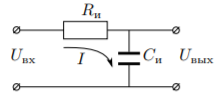
\includegraphics[width=\linewidth]{int.png}
    \caption{Интегрирующая ячейка}
    \label{fig:int}
\end{wrapfigure}

Для интегрирования в работе используется интегрирующая RC-цепочка (рис. 2).<<Входное>> напряжение от источника $U_{вх}(t)$ подаётся на последовательно соединённые резистор $R_и$ и конденсатор $C_и$. «Выходное>>
напряжение $U_{вых}(t)$ снимается с конденсатора.
 Предположим, что 1) сопротивление источника мало по сравнению с $R_и$,
  2) выходное сопротивление (сопротивление на входе осциллографа), напротив, велико: $R_{вых} > R_и$ и, наконец, 3) сопротивление $R_и$ достаточно велико, так что почти всё падение напряжения приходится на него, а $U_{вых} < U_{вх}$. В таком случае ток цепи равен I = ($U_{вх} - U_{вых}$)/$R_и \approx U_{вх}$/$R_и$, и входное и выходное сопротивление связаны соотношением
\begin{equation}
    U_{вых} = \frac{q}{C_и} = \frac{1}{C_и}\int\limits_0^t Idt \approx \frac{1}{\tau_и} \int\limits_0^t U_{вх}dt,
    \label{eq:U_ext}
\end{equation}
где $\tau_и=R_иC_и$ - постоянная времени RC - цепочки. Для индукции поля из ($\ref{eq:|B|}$) получаем 
\begin{equation}
    |B|=\frac{1}{SN}\int U_{вх} dt=\frac{\tau_и}{SN}U_{вых}.
    \label{eq:|B|new}
\end{equation}

\textbf{Замечание.} Уточним критерий применимости соотношения ($\ref{eq:U_ext}$). Пусть на вход интегрирующей ячейки подан синусоидальный сигнал с частотой $\omega_0$. Тогда, пользуясь методом комплексных амплитуд, нетрудно найти отношение амплитуд входного и выходного напряжений:
\begin{equation}
    \frac{U_{вых}}{U_{вх}}=\frac{1/\omega_0C}{\sqrt{R^2+1/(\omega_0C)^2}}.
\end{equation}
Тогда неравенство $U_{вых} \ll U_{вх}$ реализуется, если 
\begin{equation}
    \tau \equiv RC\gg \frac{1}{\omega_0}
\end{equation}
(импеданс конденсатора мал по сравнению сопротивлением резистора).
В таком случае для синусоидального сигнала имеем
\begin{equation}
    \frac{U_{вых}}{U_{вх}}\approx\frac{1}{\omega_0\tau}.
\end{equation}
В общем случае, если $\omega_0$ — частота самой низкой гармоники в спектре
произвольного входного сигнала, то при $\omega_0\tau \gg 1$ неравенство $U_{вых} \ll U_{вх}$ выполняется на любой частоте $\omega > \omega_0$.

\section{Экспериментальная установка}
Схема установки изображена на Рис. $\ref{fig:scheme}$. Напряжение сети (220 В,
50 Гц) с помощью трансформаторного блока Т, состоящего из регулировочного автотрансформатора и разделительного понижающего трансформатора, подаётся на намагничивающую обмотку $N_0$ исследуемого образца.
\begin{figure}[h!]
    \centering
    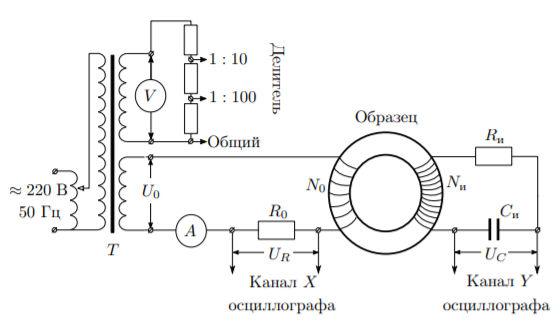
\includegraphics{scheme.png}
    \caption{ Схема установки для исследования намагничивания образцов}
    \label{fig:scheme}
\end{figure}

В цепь намагничивающей катушки, на которую подаётся некоторое
напряжение $U_0$, последовательно включено сопротивление $R_0$. Напряжение на $R_0$, равное $U_R$= $R_0I_0$, где $I_0$ — ток в намагничивающей обмотке $N_0$, подаётся на канал X осциллографа. Связь напряжённости H в
образце и тока $I_0$ рассчитывается по теореме о циркуляции. 
Действующее значение переменного тока в обмотке $N_0$ измеряется амперметром A.
Для измерения магнитной индукции B с измерительной обмотки $N_и$
на вход RC-цепочки подаётся напряжение $U_и$ ($U_{вх}$), пропорциональное
производной dB/dt. С интегрирующей ёмкости $C_и$ снимается напряжение $U_C$ ($U_{вых}$), пропорциональное величине B, и подаётся на вход Y
осциллографа. Значение индукции поля B рассчитывается по формуле ($\ref{eq:|B|new}$).
Замкнутая кривая, возникающая на экране, воспроизводит в некотором масштабе (различном для осей X и Y) петлю гистерезиса. Чтобы придать этой кривой количественный смысл, необходимо установить
масштабы изображения, т. е. провести калибровку каналов X и Y осциллографа.

\section{Ход работы}
\begin{enumerate}
    \item 

     Соберем схему согласно Рис. $\ref{fig:scheme}$. Подберем ток питания в намагничивающей обмотке с помощью автотрансформатора и коэффициенты усиления ЭО таким образом, чтобы предельная петля гистерезиса занимала большую часть экрана. Приведем характерные значения катушек разных материалов в таблице:
\begin{table}[h!]
\centering
\begin{tabular}{|c|c|c|c|c|}
\hline
& $N_0$, витков & $N_и$, витков & $S$, см$^2$ & $2\pi$ R, см \\ \hline
Феррит & 35 & 400 & 3 & 25 \\ \hline
Пермалой & 40 & 200 & 3,8 & 24 \\ \hline
\begin{tabular}[c]{@{}c@{}}Кремнистое\\ железо\end{tabular} & 35 & 350 & 1,2 & 10 \\ \hline
\end{tabular}
\caption{Характеристики катушек}
\end{table}
Для каждого образца получим передельные петли гистерезиса, по коэффициентам усиления ЭО $K_x\ и\ K_y$ рассчитаем масштабы, определим двойные амплитуды коэрцетивной силы [2x(c)] и индукции насыщения [2y(s)]. Масштабы по осям X и Y рассчитаем по формулам 
    $H=IN_0/(2\pi R),\ где\ I=K_x/R_0;\ B=R_иС_иU_{вых}/(SN_\text{и}),\ где\ U_{вых}=K_y$.    


\begin{table}[h!]
\centering
\begin{tabular}{|c|c|c|c|c|}
\hline
& ${[}2x(c){]}$, дел & ${[}2y(s){]}$, дел & $K_x$, мВ/дел & $K_y$, мВ/дел \\ \hline
Феррит & 0,6 & 4,4 & 50 & 20 \\ \hline
Пермалой & 3,6 & 4,6 & 20 & 20 \\ \hline
\begin{tabular}[c]{@{}c@{}}Кремнистое\\ железо\end{tabular} & 3,5 & 7,2 & 20 & 20 \\ \hline
\end{tabular}
\end{table}
\begin{table}[h!]
\centering
\begin{tabular}{|c|c|c|c|}
\hline
& $I$, мА & $H$, A/м дел & $B$, Тл/дел \\ \hline
Феррит & 101 & 9 & 0,07 \\ \hline
Пермалой & 215 & 26,6 & 1 \\ \hline
\begin{tabular}[c]{@{}c@{}}Кремнистое\\ железо\end{tabular} & 1580 & 90,9 & 0,5 \\ \hline
\end{tabular}
\caption{Измерения петель гистерезиса}
\end{table}

Зная масштабы по осям, можно определить значения коэрцетивной силы
и индукции насыщения.

\begin{table}[h]
\centering
\begin{tabular}{|l|l|l|l|l|l|l|l|l|l|l|}
\hline
$I эфф$, mA & 132,9 & 119,7 & 103,5 & 92,8 & 84,4 & 74,6 & 67,2 & 59,1 & 40,7 & 31,9   \\ \hline
$I$, mA & 187,9 & 169,3 & 146,3 & 131,2 & 119,4 & 105,5 & 95,0 & 83,6 & 57,6 & 45,1 \\ \hline
$U$, mB & 84 & 82 & 80 & 76 & 74 & 70 & 68 & 62 & 50 & 38  \\ \hline
$H$, A/m & 33,8 & 30,5 & 26,3 & 23,6 & 21,5 & 19,0 & 17,1 & 15,0 & 10,4 & 8,1  \\ \hline
$B$, Тл & 0,28 & 0,27 & 0,27 & 0,25 & 0,25 & 0,23 & 0,23 & 0,21 & 0,17 & 0,13  \\ \hline
$\mu$ & 6590 & 7140 & 8062 & 8538 & 9141 & 9783 & 10550 & 10937 & 12808 & 12419    \\ \hline
\end{tabular}
\caption{Результаты измерений для феррита}
\end{table}



\begin{table}[h]
\centering
\begin{tabular}{|l|l|l|l|l|l|l|l|l|l|l|}
\hline
$I эфф$, mA & 247,5 & 206,6 & 187,2 & 167,3 & 149,3 & 135,4 & 126,4 & 105,7 & 96,5  \\ \hline
$I$, mA & 350,0 & 292,2 & 264,7 & 236,6 & 211,1 & 191,5 & 178,8 & 149,5 & 136,5  \\ \hline
$U$, mB & 190 & 180 & 175 & 160 & 125 & 85 & 65 & 30 & 20  \\ \hline
$H$, A/m & 63,0 & 52,6 & 47,7 & 42,6 & 38,0 & 34,5 & 32,2 & 26,9 & 24,6  \\ \hline
$B$, Тл & 0,63 & 0,60 & 0,58 & 0,53 & 0,42 & 0,28 & 0,22 & 0,10 & 0,07   \\ \hline
$\mu$ & 8004 & 9083 & 9746 & 9971 & 8729 & 6545 & 5361 & 2959 & 2161   \\ \hline
\end{tabular}
\caption{Результаты измерений для пермаллоя}
\end{table}


Полученные значения сходятся с табличными по порядку величины.
\begin{figure}[h!]
    \centering
    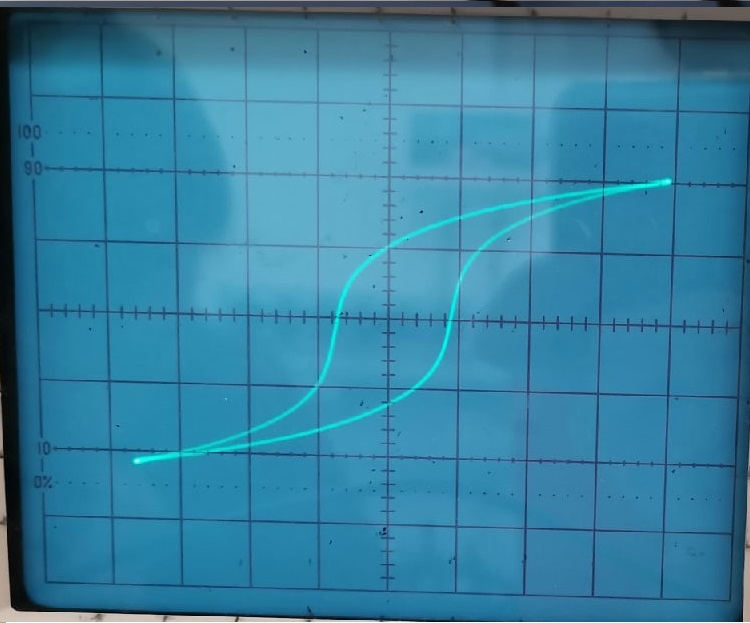
\includegraphics[width=8cm]{ferrit.jpg}
    \caption{Предельная петля гистерезиса феррита}
\end{figure}
\begin{figure}[h!]
    \centering
    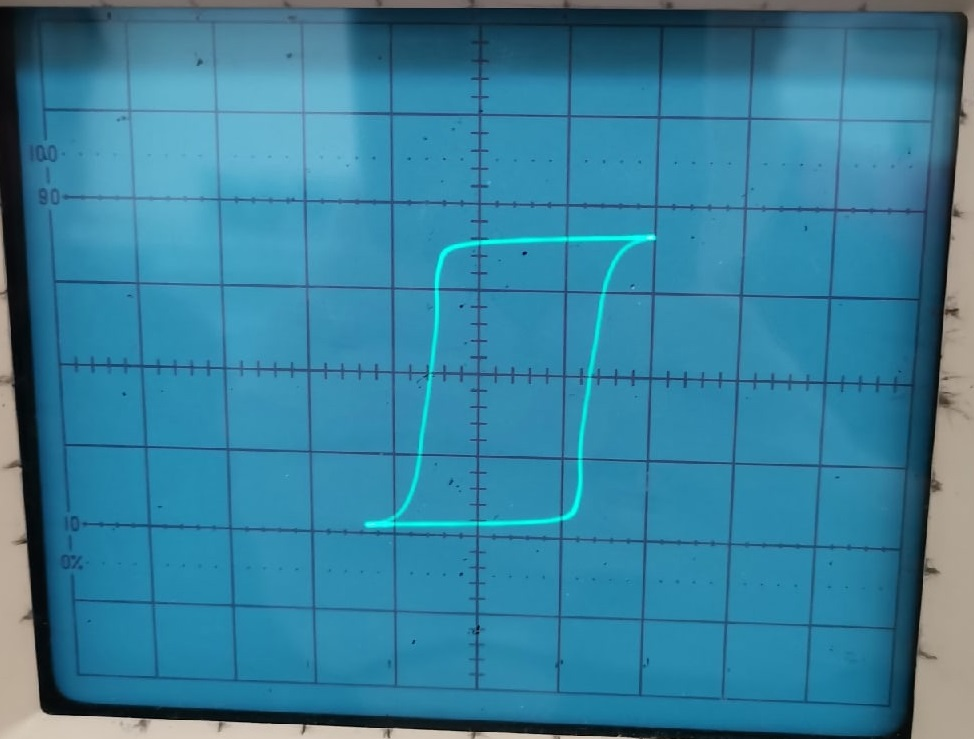
\includegraphics[width=8cm]{permalloi.jpg}
    \caption{Предельная петля гистерезиса пермаллоя}
\end{figure}
\newpage
\begin{figure}[h!]
    \centering
    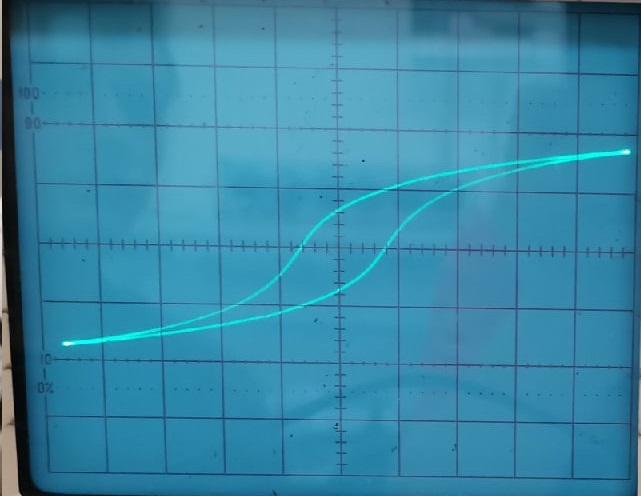
\includegraphics[width=8cm]{Si_Fe.jpg}
    \caption{Предельная петля гистерезиса для кремнистого железа}
\end{figure}

\item Проверим калибровку ЭО по оси X. Отключим намагничивающую обмотку $N_0$ от цепи, соединив оба провода, идущих к обмотке, на одной ее клемме. С помощью автотрансформатора подберем такой ток через $R_0$, при котором горизонтальная прямая занимает большую часть экрана. Рассчитаем чувствительность $m_x=0,0497\ \text{В/дел}$. Так как $m_x\approx K_x$, ЭО откалиброван по оси X корректно.

Проверим калибровку ЭО по оси Y. Для этого соединим вход Y ЭО с клеммам делителя "1:100 - земля". Не меняя рабочего коэффициента $K_Y$, подберем с помощью трансформатора напряжение, при котором вертикальная прямая занимает большую часть экрана. Подключим вольтметр V к тем же клеммам делителя и, используя измеренное $U_{\text{эф}}$, рассчитаем чувствительность $m_y=0,0499\ \text{В/дел}$. Так как $m_y\approx K_y$, ЭО откалиброван по оси Y корректно. (Все численные данные приведены на примере измерений для пермаллоя, для остальных образцов все утверждения о калибровке так же выполнены.)  

\item Проверим применимость формулы ($\ref{eq:U_ext}$). Для этого рассчитаем $\tau$ - постоянную времени RC-цепочки. Для определения напряжений на входе и выходе интегрирующей ячейки своедим вход ячейки с обмоткой "6,3 В" трансформатора. Подключим Y-вход ЭО ко входу интегрирующей ячейки и отключим X-вход ЭО. Подберем такой ток, чтобы вертикальная прямая занимала большую часть экрана, и определим входное напряжение $U_{\text{вх}}=2y\cdot K_y=7,5\ дел \cdot 1\ \text{В/дел} = 7,5\ \text{В}$. Не меняя тока, подключим Y-вход ЭО к выходу ячейки и аналогичным образом определим $U_{вых}=5,8\ дел\cdot 10\ \text{мВ/дел} = 58\ \text{мВ}$. Рассчитаем $\tau=\frac{U_{\text{вх}}}{\omega U_{\text{вых}}}=\frac{7,5}{58\cdot10^{-3}\cdot2\pi 50}=0,4116\ \text{c}$, где $\omega=2\pi\nu$. По определению $\tau_{RC}=R_иC_и=0,4\ \text{с}$. Так как $\tau\approx\tau_{RC}$, то условия применимости нашей теории выполнены.

\section{Вывод} 
Были исследованы петли гистерезиса для трех различных образцов и получены характерные величины для каждого образца, которые сошлись с табличными значениями по порядку величины. 
\end{enumerate}

\section{{Список используемой литературы}}

$\bullet$ \href{https://vk.com/doc-139677307_612194888}{Никулин М.Г. Лабораторный практикум по общей физике. Электричество и магнетизм}

$\bullet$ \href{https://mipt.ru/education/chair/physics/S_III/lab_el.php}{Описание лабораторных работ на кафедре общей физики МФТИ}

$\bullet$ \href{https://vk.com/doc-139677307_612194961}{П.В. Попов, А.А. Нозик. Обработка результатов учебного эксперимента}


\newpage
\section{{Графики}}

\begin{figure}[H]
    \centering
    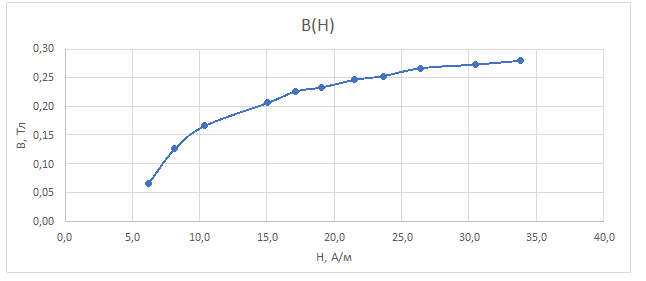
\includegraphics[scale=0.7]{феррит1.png}
    \caption{Начальная кривая намагничивания феерита}
    \label{fig:scheme}
\end{figure}

\begin{figure}[H]
    \centering
    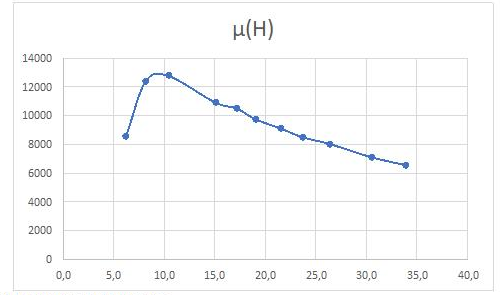
\includegraphics[scale=0.7]{феррит2.png}
    \caption{ Дифферинциальная магнитная проницаемость феерита}
    \label{fig:scheme}

    \centering
    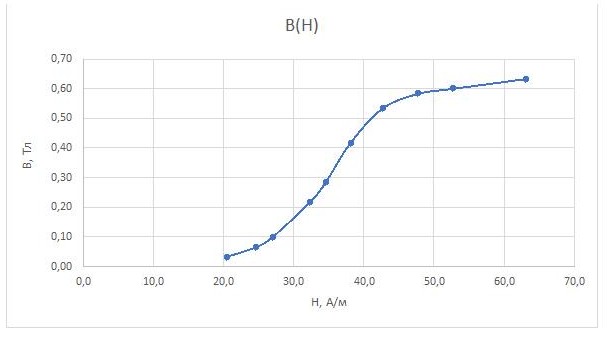
\includegraphics[scale=0.7]{пермаллой1.png}
    \caption{ Начальная кривая намагничивания пермаллоя}
    \label{fig:scheme}
\end{figure}

\begin{figure}[H]
    \centering
    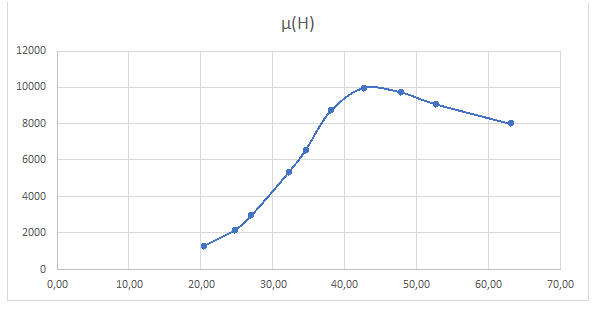
\includegraphics[scale=0.7]{пермаллой2.png}
    \caption{ Дифферинциальная магнитная проницаемость пермаллоя}
    \label{fig:scheme}
\end{figure}


\newpage

\end{document}